%!TEX root = bug-taxo.tex

\section{Introduction}

%\IEEEPARstart{T}{his} demo file is intended to serve as a ``starter file''




In order to classify the research on the different fields related to software maintenance, we can reason about types of bugs at different levels. For
example, we can group bugs based on the developers that fix
them or using information about the bugs such as crash traces.

There have been several studies (e.g., \cite{Weiß2007, Zhang2013}) that study of the factors that influence the bug fixing time.
These studies   empirically investigate the relationship between bug report attributes (description, severity, etc.) and the fixing time.
Other studies take bug analysis to another level by investigating techniques and tools for bug prediction and reproduction (e.g., \cite{Chen2013, Kim2007a, Nayrolles2015}).
These studies, however, treat all bugs as the same.
For example, a bug that requires only one fix is analyzed the same way as a bug that necessitates multiple fixes.
Similarly, if multiple bugs are fixed by modifying the exact same locations in the code, then we should investigate how these bugs are related in order to predict them in the future.
Note here that we do not refer to duplicate bugs.
Duplicate bugs are marked as duplicate (and not fixed) and only the master bug is fixed.
As a motivating example, consider Bugs \#AMQ-5066 and \#AMQ-5092 from the Apache Software Foundation bug report management system (used to build one of the datasets in this paper).
Bug \#AMQ-5066 was reported on February 19, 2014 and solved with a patch provided by the reporter.
The solution involves a relatively complex patch that modifies {\tt MQTTProtocolConverter.java}, {\tt MQTTSubscription.java} and {\tt MQTTTest.java} files.
The description of the bug is as follows:
\\ \\
{\it When a client sends a SUBSCRIBE message with the same Topic/Filter as a previous SUBSCRIBE message but a different QoS, the Server MUST discard the older subscription, and resend all retained messages limited to the new Subscription QoS.}
\\ \\
A few months later, another bug, Bug \#AMQ-5092 was reported:
\\ \\
{\it MQTT protocol converters does not correctly generate unique packet ids for retained and non-retained publish messages sent to clients.
[...] Although retained messages published on creation of client subscriptions are copies of retained messages, they must carry a unique packet id when dispatched to clients.
ActiveMQ re-uses the retained message's packet id, which makes it difficult to  acknowledge these messages when wildcard topics are used.
ActiveMQ also sends the same non-retained message multiple times for every matching subscription for overlapping subscriptions.
These messages also re-use the publisher's message id as the packet id, which breaks client acknowledgment.}
\\ \\
This bug was assigned and fixed by a different person than the one who fixed bug \#AMQ-5066.
The fix consists of modifying slightly the same lines of the code in the exact files used to fix Bug \#AMQ-5066.
In fact, Bug \#5092 could have been avoided altogether if the first developer provided a more comprehensive fix to \#AMQ-5066 (a task that is easier said than done).
These two bugs are not duplicates since, according to their description, they deal with different types of problems and yet they can be fixed by providing a similar patch.
In other words, the failures are different while the root causes (faults in the code) are more or less the same.
From the bug handling perspective, if we can develop a way to detect such related bug reports during triaging then we can achieve considerable time saving in the way bug reports are processed, for example, by assigning them to the same developers.
We also conjecture that detecting such related bugs can help with other tasks such as bug reproduction.
We can  reuse the reproduction of an already fixed bug to reproduce an incoming and related bug.

Our aim is not to improve testing as it is the case in the work of Eldh \cite{Eldh2001} and Hamill et al.\cite{Hamill2014}.
Our objective is to propose a classification that can allow researchers in the filed of mining bug 9 repositiories to use the taxonomy as a new criterion in triaging, prediction, and reproduction of bugs.
By analogy, we can look at the proposed bug taxonomy in a similar way as the clone taxonomy presented by Kapser and Godfrey \cite{CoryKapser}.
The authors proposed seven types of source code clones and then conducted a case study, using their classification, on the file system module of the Linux operating system.
This clone taxonomy continues to be used by researchers to build better approaches for detecting a given clone type and being able to effectively compare approaches with each other.

We are interested in bugs that share similar fixes.
By a fix, we mean a modification (adding or deleting lines of
code) to an exiting file that is used to solve the bug. With this
in mind, the relationship between bugs and fixes can be
modeled using the UML diagram in Figure \ref{fig:bug-taxo-diag}. The diagram
only includes bugs that are fixed. From this figure, we can
think of four instances of this diagram, which we refer to as
bug taxonomy or simply bug types (see Figure \ref{fig:bug-taxo}).



\begin{figure}[h!]
  \centering
    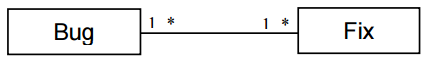
\includegraphics[scale=0.5]{media/bug-taxo-class-diag.png}
    \caption{Class diagram showing the relationship between bugs and fixed
    \label{fig:bug-taxo-diag}}
\end{figure}


\begin{figure}[h!]
  \centering
    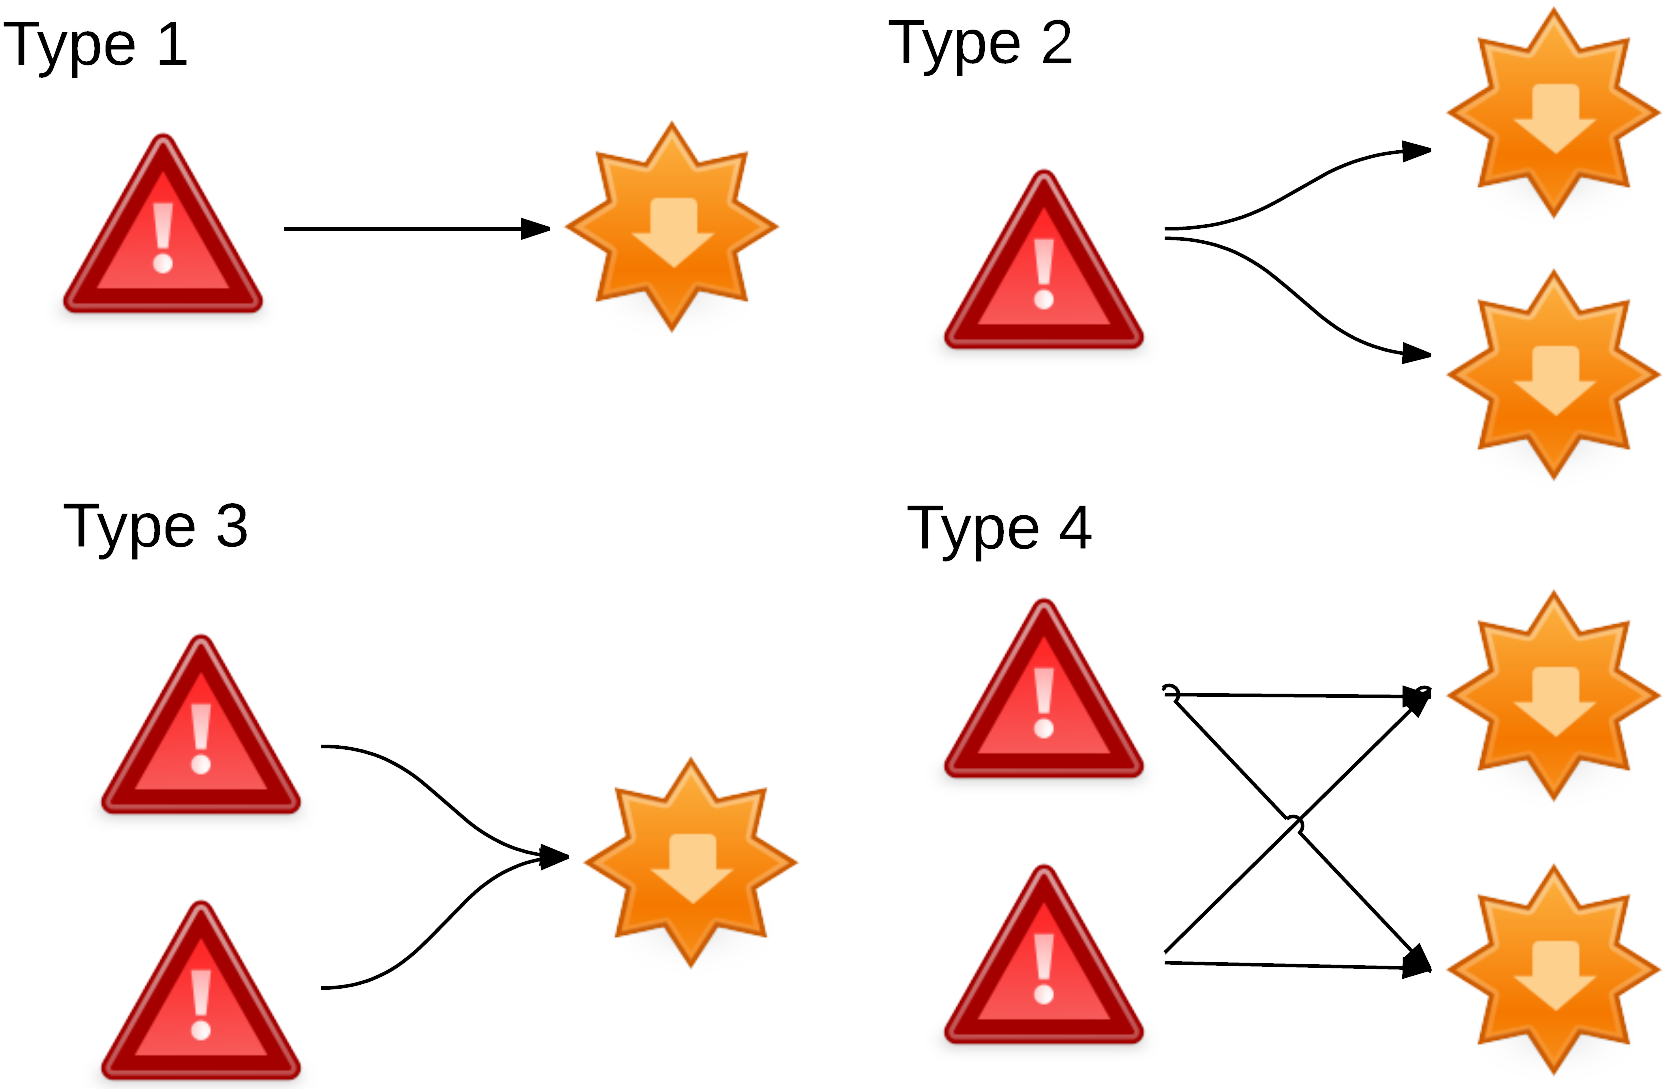
\includegraphics[scale=0.6]{media/bug-taxo.png}
    \caption{Proposed Taxonomy of Bugs
    \label{fig:bug-taxo}}
\end{figure}


The first and second types are the ones we intuitively know
about.
Type 1 refers to a bug being fixed in one single location (i.e., one file), while Type 2 refers to bugs being fixed in more than one location.
In Figure 2, only two locations are shown for the sake of clarity, but many more locations could be involved in the fix of a bug.
Type 3 refers to multiple bugs that are fixed in the exact same location.
Type 4 is an extension of Type 3, where multiple bugs are resolved by modifying the same set of locations.
Note that Type 3 and Type 4 bugs are not duplicates, they may occur when different features of the system fail due to the same root causes (faults).
We conjecture that knowing the proportions of each type of bugs in a system may provide insight into the quality of the system.
Knowing, for example, that in a given system the proportion of Type 2 and 4 bugs is high may be an indication of poor system quality since many fixes are needed to address these bugs.
In addition, the existence of a high number of Types 3 and 4 bugs calls for techniques that can effectively find bug reports related to an incoming bug during triaging.
This is similar to the many studies that exist on detection of duplicates (e.g., \cite{Runeson2007,Sun2010,Nguyen2012}), except that we are not looking for duplicates but for related bugs (bugs that are due to failures of different features of the system, caused by the same faults).
To our knowledge, there is no study that exmpirically examines bug data with these types in mind, which is the main objective of this section.
More particularly, we are interested in the following research questions:

\begin{itemize}
	\item RQ1: What are the proportions of different types of bugs?
	\item RQ2: How complex is each type of bugs?
	\item RQ3: How pertinent is a bug taxonomy?
\end{itemize}
